
\documentclass[letterpaper,hide notes,xcolor={table,svgnames},10pt]{beamer}
\def\showexamples{t}


%\usepackage[svgnames]{xcolor}

%% Demo talk
%\documentclass[letterpaper,notes=show]{beamer}

\usecolortheme{crane}
\setbeamertemplate{navigation symbols}{}

\usetheme{MyPittsburgh}
%\usetheme{Frankfurt}

%\usepackage{tipa}

\usepackage{hyperref}
\usepackage{graphicx,xspace}
\usepackage[normalem]{ulem}
\usepackage{multicol}
\usepackage{amsmath,amssymb,amsthm,graphicx,xspace}
\newcommand\SF[1]{$\bigstar$\footnote{SF: #1}}

\usepackage[default]{sourcesanspro}
\usepackage[T1]{fontenc}
\usepackage[scaled]{beramono}
\usepackage{tikzpagenodes}

\newcounter{tmpnumSlide}
\newcounter{tmpnumNote}


% old question code
%\newcommand\question[1]{{$\bigstar$ \small \onlySlide{2}{#1}}}
% \newcommand\nquestion[1]{\ifdefined \presentationonly \textcircled{?} \fi \note{\par{\Large \textbf{?}} #1}}
% \newcommand\nanswer[1]{\note{\par{\Large \textbf{A}} #1}}


 \newcommand\mnote[1]{%
   \addtocounter{tmpnumSlide}{1}
   \ifdefined\showcues {~\tiny\fbox{\arabic{tmpnumSlide}}}\fi
   \note{\setlength{\parskip}{1ex}\addtocounter{tmpnumNote}{1}\textbf{\Large \arabic{tmpnumNote}:} {#1\par}}}

\newcommand\mmnote[1]{\note{\setlength{\parskip}{1ex}#1\par}}

%\newcommand\mnote[2][]{\ifdefined\handoutwithnotes {~\tiny\fbox{#1}}\fi
% \note{\setlength{\parskip}{1ex}\textbf{\Large #1:} #2\par}}

%\newcommand\mnote[2][]{{\tiny\fbox{#1}} \note{\setlength{\parskip}{1ex}\textbf{\Large #1:} #2\par}}

\newcommand\mquestion[2]{{~\color{red}\fbox{?}}\note{\setlength{\parskip}{1ex}\par{\Large \textbf{?}} #1} \note{\setlength{\parskip}{1ex}\par{\Large \textbf{A}} #2\par}\ifdefined \presentationonly \pause \fi}

\newcommand\blackboard[1]{%
\ifdefined   \showblackboard
  {#1}
  \else {\begin{center} \fbox{\colorbox{blue!30}{%
         \begin{minipage}{.95\linewidth}%
           \hspace{\stretch{1}} Some space intentionally left blank; done at the blackboard.%
         \end{minipage}}}\end{center}}%
         \fi%
}

\newcommand{\Rplus}{\protect\hspace{-.1em}\protect\raisebox{.35ex}{\small{\small\textbf{+}}}}
\newcommand{\CPP}{\mbox{C\Rplus\Rplus}\xspace}

%\newcommand\q{\tikz \node[thick,color=black,shape=circle]{?};}
%\newcommand\q{\ifdefined \presentationonly \textcircled{?} \fi}

\usepackage{listings,listings-rust}
\lstset{basicstyle=\footnotesize\ttfamily,
	breaklines=true,
	aboveskip=15pt,
  	belowskip=15pt,
	frame=lines,
	numbers=left, basicstyle=\scriptsize, numberstyle=\tiny, stepnumber=0, numbersep=2pt
}

\usepackage{siunitx}
\newcommand\sius[1]{\num[group-separator = {,}]{#1}\si{\micro\second}}
\newcommand\sims[1]{\num[group-separator = {,}]{#1}\si{\milli\second}}
\newcommand\sins[1]{\num[group-separator = {,}]{#1}\si{\nano\second}}
\sisetup{group-separator = {,}, group-digits = true}

%% -------------------- tikz --------------------
\usepackage{tikz}
\usetikzlibrary{positioning}
\usetikzlibrary{arrows,backgrounds,automata,decorations.shapes,decorations.pathmorphing,decorations.markings,decorations.text,decorations.pathreplacing}

\tikzstyle{place}=[circle,draw=blue!50,fill=blue!20,thick, inner sep=0pt,minimum size=6mm]
\tikzstyle{transition}=[rectangle,draw=black!50,fill=black!20,thick, inner sep=0pt,minimum size=4mm]

\tikzstyle{block}=[rectangle,draw=black, thick, inner sep=5pt]
\tikzstyle{bullet}=[circle,draw=black, fill=black, thin, inner sep=2pt]

\tikzstyle{pre}=[<-,shorten <=1pt,>=stealth',semithick]
\tikzstyle{post}=[->,shorten >=1pt,>=stealth',semithick]
\tikzstyle{bi}=[<->,shorten >=1pt,shorten <=1pt, >=stealth',semithick]

\tikzstyle{mut}=[-,>=stealth',semithick]

\tikzstyle{treereset}=[dashed,->, shorten >=1pt,>=stealth',thin]

\usepackage{ifmtarg}
\usepackage{xifthen}
\makeatletter
% new counter to now which frame it is within the sequence
\newcounter{multiframecounter}
% initialize buffer for previously used frame title
\gdef\lastframetitle{\textit{undefined}}
% new environment for a multi-frame
\newenvironment{multiframe}[1][]{%
\ifthenelse{\isempty{#1}}{%
% if no frame title was set via optional parameter,
% only increase sequence counter by 1
\addtocounter{multiframecounter}{1}%
}{%
% new frame title has been provided, thus
% reset sequence counter to 1 and buffer frame title for later use
\setcounter{multiframecounter}{1}%
\gdef\lastframetitle{#1}%
}%
% start conventional frame environment and
% automatically set frame title followed by sequence counter
\begin{frame}%
\frametitle{\lastframetitle~{\normalfont(\arabic{multiframecounter})}}%
}{%
\end{frame}%
}
\makeatother

\makeatletter
\newdimen\tu@tmpa%
\newdimen\ydiffl%
\newdimen\xdiffl%
\newcommand\ydiff[2]{%
    \coordinate (tmpnamea) at (#1);%
    \coordinate (tmpnameb) at (#2);%
    \pgfextracty{\tu@tmpa}{\pgfpointanchor{tmpnamea}{center}}%
    \pgfextracty{\ydiffl}{\pgfpointanchor{tmpnameb}{center}}%
    \advance\ydiffl by -\tu@tmpa%
}
\newcommand\xdiff[2]{%
    \coordinate (tmpnamea) at (#1);%
    \coordinate (tmpnameb) at (#2);%
    \pgfextractx{\tu@tmpa}{\pgfpointanchor{tmpnamea}{center}}%
    \pgfextractx{\xdiffl}{\pgfpointanchor{tmpnameb}{center}}%
    \advance\xdiffl by -\tu@tmpa%
}
\makeatother
\newcommand{\copyrightbox}[3][r]{%
\begin{tikzpicture}%
\node[inner sep=0pt,minimum size=2em](ciimage){#2};
\usefont{OT1}{phv}{n}{n}\fontsize{4}{4}\selectfont
\ydiff{ciimage.south}{ciimage.north}
\xdiff{ciimage.west}{ciimage.east}
\ifthenelse{\equal{#1}{r}}{%
\node[inner sep=0pt,right=1ex of ciimage.south east,anchor=north west,rotate=90]%
{\raggedleft\color{black!50}\parbox{\the\ydiffl}{\raggedright{}#3}};%
}{%
\ifthenelse{\equal{#1}{l}}{%
\node[inner sep=0pt,right=1ex of ciimage.south west,anchor=south west,rotate=90]%
{\raggedleft\color{black!50}\parbox{\the\ydiffl}{\raggedright{}#3}};%
}{%
\node[inner sep=0pt,below=1ex of ciimage.south west,anchor=north west]%
{\raggedleft\color{black!50}\parbox{\the\xdiffl}{\raggedright{}#3}};%
}
}
\end{tikzpicture}
}


%% --------------------

%\usepackage[excludeor]{everyhook}
%\PushPreHook{par}{\setbox0=\lastbox\llap{MUH}}\box0}

%\vspace*{\stretch{1}

%\setbox0=\lastbox \llap{\textbullet\enskip}\box0}

\setlength{\parskip}{\fill}

\newcommand\noskips{\setlength{\parskip}{1ex}}
\newcommand\doskips{\setlength{\parskip}{\fill}}

\newcommand\xx{\par\vspace*{\stretch{1}}\par}
\newcommand\xxs{\par\vspace*{2ex}\par}
\newcommand\tuple[1]{\langle #1 \rangle}
\newcommand\code[1]{{\sf \footnotesize #1}}
\newcommand\ex[1]{\uline{Example:} \ifdefined \presentationonly \pause \fi
  \ifdefined\showexamples#1\xspace\else{\uline{\hspace*{2cm}}}\fi}

\newcommand\ceil[1]{\lceil #1 \rceil}


\AtBeginSection[]
{
   \begin{frame}
       \frametitle{Outline}
       \tableofcontents[currentsection]
   \end{frame}
}



\pgfdeclarelayer{edgelayer}
\pgfdeclarelayer{nodelayer}
\pgfsetlayers{edgelayer,nodelayer,main}

\tikzstyle{none}=[inner sep=0pt]
\tikzstyle{rn}=[circle,fill=Red,draw=Black,line width=0.8 pt]
\tikzstyle{gn}=[circle,fill=Lime,draw=Black,line width=0.8 pt]
\tikzstyle{yn}=[circle,fill=Yellow,draw=Black,line width=0.8 pt]
\tikzstyle{empty}=[circle,fill=White,draw=Black]
\tikzstyle{bw} = [rectangle, draw, fill=blue!20, 
    text width=4em, text centered, rounded corners, minimum height=2em]
    
    \newcommand{\CcNote}[1]{% longname
	This work is licensed under the \textit{Creative Commons #1 3.0 License}.%
}
\newcommand{\CcImageBy}[1]{%
	\includegraphics[scale=#1]{creative_commons/cc_by_30.pdf}%
}
\newcommand{\CcImageSa}[1]{%
	\includegraphics[scale=#1]{creative_commons/cc_sa_30.pdf}%
}
\newcommand{\CcImageNc}[1]{%
	\includegraphics[scale=#1]{creative_commons/cc_nc_30.pdf}%
}
\newcommand{\CcGroupBySa}[2]{% zoom, gap
	\CcImageBy{#1}\hspace*{#2}\CcImageNc{#1}\hspace*{#2}\CcImageSa{#1}%
}
\newcommand{\CcLongnameByNcSa}{Attribution-NonCommercial-ShareAlike}

\newenvironment{changemargin}[1]{% 
  \begin{list}{}{% 
    \setlength{\topsep}{0pt}% 
    \setlength{\leftmargin}{#1}% 
    \setlength{\rightmargin}{1em}
    \setlength{\listparindent}{\parindent}% 
    \setlength{\itemindent}{\parindent}% 
    \setlength{\parsep}{\parskip}% 
  }% 
  \item[]}{\end{list}} 




\title{Lecture 23 --- GPU Programming Continued }

\author{Jeff Zarnett \\ \small \texttt{jzarnett@uwaterloo.ca}}
\institute{Department of Electrical and Computer Engineering \\
  University of Waterloo}
\date{\today}


\begin{document}

\begin{frame}
  \titlepage

\end{frame}


\begin{frame}
\frametitle{The Host Code}

We've learned about how a kernel works and a bit about how to write one. 

The next part is the host code.

Now, fortunately, we don't have to write the whole program in \CPP~ or C, even though the kernel has to be written in the CUDA variant. 

We're going to use the Rustacuda library!
\end{frame}


\begin{frame}[fragile]
\frametitle{Rust Host Code Example}
\begin{lstlisting}[language=Rust]
#[macro_use]
extern crate rustacuda;

use rustacuda::prelude::*;
use std::error::Error;
use std::ffi::CString;

fn main() -> Result<(), Box<dyn Error>> {
    // Set up the context, load the module, and create a stream to run kernels in.
    rustacuda::init(CudaFlags::empty())?;
    let device = Device::get_device(0)?;
    let _ctx = Context::create_and_push(ContextFlags::MAP_HOST | ContextFlags::SCHED_AUTO, device)?;

    let ptx = CString::new(include_str!("../resources/add.ptx"))?;
    let module = Module::load_from_string(&ptx)?;
    let stream = Stream::new(StreamFlags::NON_BLOCKING, None)?;
    
    // Create buffers for data
    let mut in_x = DeviceBuffer::from_slice(&[1.0f32; 10])?;
    let mut in_y = DeviceBuffer::from_slice(&[2.0f32; 10])?;
    let mut out_1 = DeviceBuffer::from_slice(&[0.0f32; 10])?;
    let mut out_2 = DeviceBuffer::from_slice(&[0.0f32; 10])?;
\end{lstlisting}

\end{frame}


\begin{frame}[fragile]
\frametitle{Rust Host Code Example}
\begin{lstlisting}[language=Rust]
    // This kernel adds each element in `in_x` and `in_y` and writes the result into `out`.
    unsafe {
        // Launch the kernel with one block of one thread, no dynamic shared memory on `stream`.
        let result = launch!(module.sum<<<1, 1, 0, stream>>>(
            in_x.as_device_ptr(),
            in_y.as_device_ptr(),
            out_1.as_device_ptr(),
            out_1.len()
        ));
        result?;
    }

    // Kernel launches are asynchronous, so we wait for the kernels to finish executing.
    stream.synchronize()?;
\end{lstlisting}

\begin{center}
	
\includegraphics[width=0.4\textwidth]{images/launch-sw.jpg}
\end{center}

\end{frame}


\begin{frame}[fragile]
\frametitle{Rust Host Code Example}
\begin{lstlisting}[language=Rust]

    // Copy the results back to host memory
    let mut out_host = [0.0f32; 20];
    out_1.copy_to(&mut out_host[0..10])?;
    out_2.copy_to(&mut out_host[10..20])?;

    for x in out_host.iter() {
        assert_eq!(3.0 as u32, *x as u32);
    }

    println!("Launched kernel successfully.");
    Ok(())
}
\end{lstlisting}
\vspace{-1em}
\begin{center}
	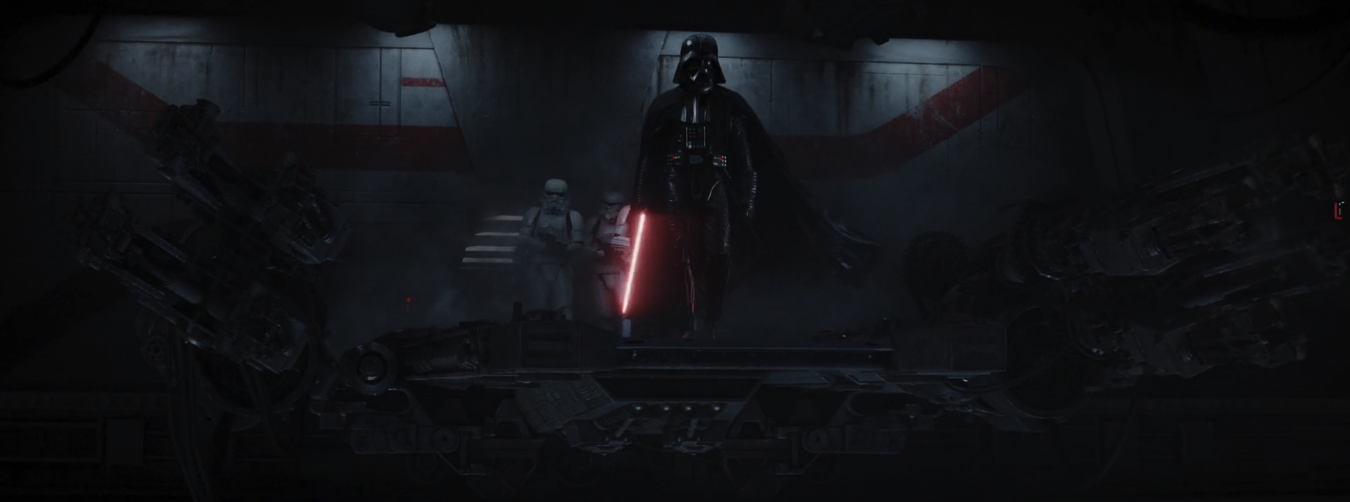
\includegraphics[width=0.8\textwidth]{images/vader-rogue-one.png}
\end{center}

\end{frame}


\begin{frame}[fragile]
\frametitle{Corresponding Kernel}

\begin{lstlisting}[language=C]
extern "C" __constant__ int my_constant = 314;

extern "C" __global__ void sum(const float* x, const float* y, float* out, int count) {
    for (int i = blockIdx.x * blockDim.x + threadIdx.x; i < count; i += blockDim.x * gridDim.x) {
        out[i] = x[i] + y[i];
    }
}
\end{lstlisting}


\begin{center}
	
\includegraphics[width=0.8\textwidth]{images/tantive-iv.png}
\end{center}
\end{frame}

\begin{frame}[fragile]
\frametitle{N-Body Problem}

Let's take a look at the N-Body Problem code in the repo.

\end{frame}


\begin{frame}
\frametitle{Results}

That's great, but how much does it speed up? 

I ran this on ecetesla1.

With 100~000 points:
\begin{itemize}
	\item \texttt{nbody} (sequential, no approximations): 40.3 seconds
	\item \texttt{nbody-parallel} (parallel, no approximations): 5.3 seconds
	\item \texttt{nbody-cuda} (parallel, no approximations): 9.5 seconds
\end{itemize}

\end{frame}


\begin{frame}
\frametitle{Wait a Minute}

\begin{center}
	
\includegraphics[width=0.9\textwidth]{images/chosenone.png}
\end{center}

 That's worse than the CPU version. 
 

\end{frame}

\begin{frame}
\frametitle{Kylo Ren is very Meme-Able}

Theory: 100~000 points is not enough to overcome the overhead of setup and transferring data to and from the device. 
  
\begin{center}
	
\includegraphics[width=0.9\textwidth]{images/more.png}
\end{center}
  
\end{frame}

\begin{frame}
\frametitle{Sequel Memes!}

\begin{center}
	
\includegraphics[width=0.8\textwidth]{images/wrong.png}
\end{center}

This turned out to be incorrect.

Most of the time was going to the kernel execution of the \texttt{calculate\_forces} -- as expected?

\end{frame}


\begin{frame}
\frametitle{This Was Important}

\begin{center}
	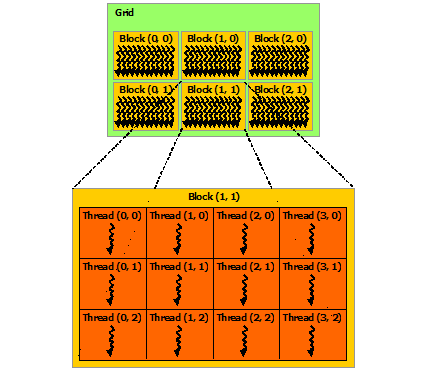
\includegraphics[width=0.45\textwidth]{images/grid-of-thread-blocks.png}
\end{center}

The documentation isn't super great about how grids and blocks work.

A lot of the guidance on the internet says is ``experiment and try''. 

\end{frame}


\begin{frame}
\frametitle{Grid Guidance}

 The initial approach that I wrote had each work-item be its own grid. 
 
 That's inefficient, because we're not taking advantage of all the hardware that's available (the warp hardware). 
 
 The advice that I can find says the number of threads per block should always be a multiple of 32 with a maximum of 512 (or perhaps 1024). 
 
 The second guidance I can find is that numbers like 256 and 128 are good ones to start with, and you can tweak it as you need. 
 
 Then you have to adjust the grid size: divide the number of points by the threads per block to give the number of blocks.

\end{frame}


\begin{frame}[fragile]
\frametitle{Change the Launch}

\begin{lstlisting}[language=Rust]
        let result = launch!(module.calculate_forces<<<(NUM_POINTS/256) + 1, 256, 0, stream>>>(
            points.as_device_ptr(),
            accel.as_device_ptr(),
            points.len()
        ));
        result?;
\end{lstlisting}

I did have to add a +1 to the number of blocks, because 100~000 does not divide evenly by 256.

\end{frame}


\begin{frame}
\frametitle{Kernel Crash}

 But just running it as-is didn't work (and led to the kernel crashing. Why? 
 
 Because the indexing strategy that I used contained only the reference to the block index \texttt{blockIdx.x}. 
 
 That's fine in the scenario where every work-item gets its own block, but that's no longer the case now: 256 work-items (points) now share each block.


\end{frame}


\begin{frame}[fragile]
\frametitle{Updated Kernel}

\begin{lstlisting}[language=C++]
extern "C" __global__ void calculate_forces(const float4* positions, float3* accelerations, int num_points) {
    int idx = threadIdx.x + blockIdx.x * blockDim.x;
    if (idx >= num_points) {
        return;
    }
    float4 current = positions[idx];
    float3 acc = accelerations[idx];

    for (int i = 0; i < num_points; i++) {
        body_body_interaction(current, positions[i], &acc);
    }
    accelerations[idx] = acc;
}
\end{lstlisting}

\end{frame}


\begin{frame}
\frametitle{Did it work?}

With 100~000 points:

\begin{center}
	
\includegraphics[width=0.7\textwidth]{images/power.png}
\end{center}

\begin{itemize}
	\item \texttt{nbody} (sequential, no approximations): 40.3 seconds
	\item \texttt{nbody-parallel} (parallel, no approximations): 5.3 seconds
	\item \texttt{nbody-cuda} (parallel, no approximations): 9.5 seconds
	\item \textbf{\texttt{nbody-cuda-grid} (parallel, no approx., grid): 1.65 seconds}
\end{itemize}

 Now that's a lot better!

\end{frame}

\end{document}

